%\documentclass[preprint2,numberedappendix,tighten,twocolappendix]{aastex6}  % USE THIS TO MAKE BIB, THEN FORMAT USING EMULATEAPJ
\documentclass[twocolumn,apj,numberedappendix]{emulateapj}
\shorttitle{Adding Sensitivity to 21\,cm Inteferometric Probes of Reionization}
\shortauthors{Zhang, Liu \&Parsons}
\usepackage{float}
\usepackage{amsmath}
\usepackage{graphicx}
\usepackage[figuresright]{rotating}
%\usepackage{rotating}
\usepackage{natbib}
\usepackage{gensymb}
%\usepackage{pdflscape}
%\usepackage{lscape}
\usepackage{ctable}
\citestyle{aa}
\renewcommand\[{\begin{equation}}
\renewcommand\]{\end{equation}}
\graphicspath{{../figures/}}

\begin{document}

\title{A Generalized Visbility to Power-Spectrum Framework for 21\,cm Inteferometric Probes of Reionizations}

%\maketitle
\author{
Yunfan Gerry Zhang \altaffilmark{1},
Adrian Liu \altaffilmark{1, 2},
Aaron R. Parsons\altaffilmark{1, 2}
}

\altaffiltext{1}{Astronomy Dept., U. California, Berkeley, CA}
\altaffiltext{2}{Radio Astronomy Lab., U. California, Berkeley, CA}

\begin{abstract}
Measuring the cosmological 21\,cm power spectrum with radio interferometers requires high sensitivity. Many modern low-frequency interferometers are thus designed with antennas placed on regular grid to maximize redundancy. Current visibility-based power spectrum pipelines, though shown to ease control of systematics, lack the ability to include partial redundancy. We introduce a method to include partial redundancy in such power spectrum pipelines of drift-scan arrays. Our method pairs baselines to cross-multiply at a time lag, and quantifies the sensitivity contributions of each pair of baselines. 
Using the 128-element configurations and beams of the Donald C. Backer Precision Array for Probing the Epoch of Reionization (PAPER-128), and 4 planned versions of the Hydrogen Epoch of Reionization Array (HERA), we illustrate how our method applies to different arrays and predict the sensitivity improvements of including each baseline pairs. We show that inclusion of partially redundant baselines 
would account for $20\%$ to $60\%$ of the sensitivity of PAPER-128 and different configurations of HERA. 
\end{abstract}

\section{Introduction}

The epoch of reionization represents the last key
stage of our Universe's early evolution. Study of this event stands at
the intersection of cosmology and astrophysics. Understanding this
event not only serves as a scientific goal
of its own, but also as a gateway to crucial information
regarding fundamental physics of inflation, neutrino mass and phenomenology
of the first stars and galaxies (e.g. \citealt{LiuOpticalDepth, Liu2016b, Mao2008, DEw21cm, Bull2015, Oyama20131186}). 

Observational studies of reionization, including Gunn-Peterson measurements of quasi-stellar objects \citep{Fan2006} and cosmic microwave background temperature and anisotropy measurements (CMB;\citealt{Planck2016}), the Kinetic Sunyaev-Zeldo'vich effect \citep{kszpatchy} and Lyman alpha emitter clustering \citep{mcquinnLyA} have given us indications of the rough time-frame of reionization, but only limited constraints on the finer spatial and temporal structures. A surge of recent radio-astronomical experiments of reionization focus on measuring the ``spin-flip'' transition of neutral
hydrogen of characteristic wavelength 21\,cm \citep{Furlanetto2006181,PritchardLoeb}.
The 21\,cm brightness temperature is a direct tracer of neutral hydrogen through the epoch of reionization, and thus tomography of the 21\,cm line is a direct measurement of the full temporal and spatial variations of this event. 
Before realizing of full-scale 21\,cm tomography, many current radio interferometric efforts
aim to measure the spatial power spectrum of 21\,cm brightness temperature fluctuations.
Current-generation instruments include the Donald C. Backer Precision Array for Probing
the Epoch of Reionization (PAPER; \citealt{Ali2015,paper32}), Murchison
Widefield Array (MWA; \citealt{Bowman2013, Tingay2013}), Low Frequency Array (LOFAR; \citealt{LOFAR}). Next-generation instruments include the Hydrogen Epoch of Reionization
Array (HERA; e.g. \citealt{HERA,HERAconfiguration,HERABEAM1,HERADISH2})  under construction, 
and the Square Kilometer Array Low (SKA-low; e.g. \citealt{SKA1}) currently in planning stages. 

The highly redshifted 21\,cm signal is faint and diffuse, in contrast to the localized bright sources targeted by many traditional radio telescopes.  Current 21\,cm experiments are sensitivity-starved, with the sensitivity requirement further increased considering the foreground contaminations 5 orders of magnitude brighter than the cosmological signal of interest. Low-frequency radio interferometers aiming to measure the 21\,cm signal are thus designed differently from traditional instruments. Specially designed arrays such as PAPER and HERA feature multiple copies of the same baselines to repeatedly measure the same Fourier signal to increase sensitivity \citep{first-paper}. To satisfy the sensitivity need, modern arrays are large. Ranging upwards from 100 elements, these arrays are typically of the drift-scan type to limit cost.

Analysis pipelines for the 21\,cm power spectrum typically fall into two categories. In the first, images are formed in Fourier domain through rotation synthesis, followed by a foreground mitigation step to construct a power spectrum. An alternative technique works directly with visibilities from baselines, delay-transforming and cross-multiplying them to form the power spectrum. This technique avoids many systematics associated with combining data from different baselines and tracks the native sampling of the interferometer. An example of the visibility-based pipeline was presented in \cite{Ali2015}, which provides the newest upper limit to the power spectrum
measurements with the 64-element version of PAPER (henceforth as PAPER-64). However, one disadvantage of existing visibility-based pipelines is their lack of use of partial redundancy. Baselines of different lengths and orientations contain partially redundant information. While imaging based power-spectrum pipelines naturally includes all redundancy information, visibility-based pipelines so far only cross multiply fully redundant baselines, i.e. baselines of the same length and orientation.

Visibility-based pipelines are not fundamentally limited from using partially redundant baselines. In fact, most sensitivity forecasts to date do include partial redundancy \citep{Pobersens, HERA, JoshAntPos}. Recently, \cite{wterm} proposed a visibility-based approach to extract power spectrum from partially redundant baselines in sky-tracking measurements. Arrays capable of such tracking include MWA and LOFAR. Our work parallels this effort by focusing on drift-scan arrays that do not have tracking capabilities, such as PAPER, HERA and potentially SKA-low.

The Earth's rotation causes the baselines in a drift-scan array to pick up different modes of the sky with time. Rotation-synthesis makes use of the rotation-induced $uv$ coverage map to form image. In a visibility based pipeline, we can extract the same rotation-induced redundancy. In this point of view, baselines that are slightly different in length and orientation
``rotate into'' each other at a time delay. We can thus cross-multiply time-shifted visibilities, with the proper weighting, to form power spectra.  Due to the large number of elements of modern arrays (upward of 100), the task of cross-multiplying every baseline against every other, scaling as number of array elements to the fourth power, can be computationally formidable, and many pairs of baselines provide only negligible redundancy information. Our contribution is thus twofold. First we introduce a formalism to include pairs of partially-redundant baselines in a visibility based power spectrum pipeline. Secondly we show how to use the formalism to automatically pre-select baseline pairs and time offsets, making the problem computationally efficient. More precisely, our formalism allows one to simultaneously identify the baselines that give good
redundancy, find the time offset that corresponds to maximal redundancy for a given pair of baselines, and quantify the sensitivity associated with cross multiplying
such a pair of partially redundant baselines, which in turns is used as weight to combine measurements in a power spectrum pipeline. 

%[TODO: this paragraph would potentially be promoted to a section] By using pairs of baselines, we also reduce additional mode mixing. As discussed in \cite{Hazelton2013}, the varying shapes of overlapping regions in $uv$ space of all contributing baselines lead to chromaticities in the response. By considering only pairs of baselines, we fix shapes of overlapping regions, and only let their sizes vary with frequency, just as in the case of fully redundant baselines.  



The rest of this paper is organized as follows. In section 2 we introduce some terminology and notation used in the rest of the paper. In section
3 we introduce the formalism for weighting partially redundant baselines.
In section 4 we present numerical tests of
this technique as well as the expected sensitivity improvement
 this method provides for HERA and PAPER-128 pipelines, and with section 5 we conclude. 

\section{Notation and Terminology}

In order to avoid confusion and ambiguity for the rest of this paper, we
introduce some terminology that may differ from what is commonly found in the literature. 

We make the distinction between a \textit{baseline}, which corresponds to two specific antennas, and a \textit{class of baselines}, which refers to all baselines of the same length and orientation in a given array. 
Baselines of the same class are traditionally called
``redundant baselines'', because they measure the same Fourier mode
in the sky.  We shall call baselines in the same class \textit{equivalent baselines}, and reserve the word \textit{redundancy} of two baselines in reference to a variable function of the relative time-offsets of their visibility time series. With this terminology, two equivalent
baselines are fully redundant with each other simultaneously at all
times. Non-equivalent baselines also have partial redundancy, and the redundancy can be maximized if their
respected time series are shifted with respect to one another by some delay. 

\begin{figure}[H]
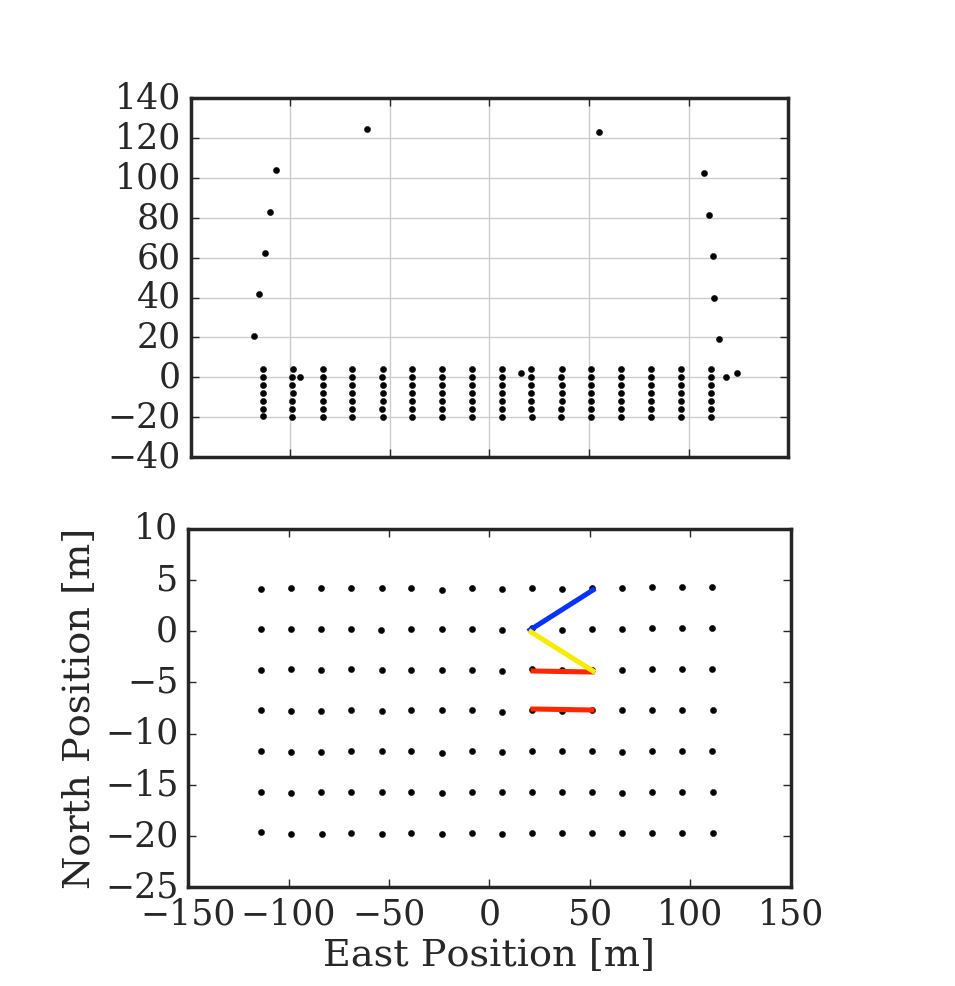
\includegraphics[width=\linewidth]{antconfig}

\caption{The PAPER128 layout. Each dot corresponds to the location of
an antenna. The top panel shows the antenna positions drawn to scale;
the bottom panel show the antenna labels and distances of the 112-element grid, in other words excluding the outrigger antennas.
The numbering of the antennas in the bottom panel are original labels
during instrument assembly and does not bear significant
meaning. In the bottom panel, the two baselines marked with red segments are example of an equivalent pair, each with antennas separated by 2 units east and 0 unit north. Similarly,
the baselines marked in blue and yellow are examples
of classes that , due to the small North-South separation within the grid (see top panel), are expected to be nearly equivalent to the red baselines. }
\label{fig:AntPos}
\end{figure}

We shall use the 128-element PAPER array (henceforth as PAPER-128) to motivate our formalism and demonstrate our method, and extend our results to several HERA configurations in Sec \ref{sec:arrconf}. 
The PAPER array is located in the Karoo desert in South Africa (30:43:17.5
S, 21:25:41.8 E). The layout pattern with antenna labels is shown
in Fig. \ref{fig:AntPos}. The array consists of a 112-element core is a rectangular grid, and 16 "outriggers" used primarily to aid calibration.  In the bottom panel, the two baselines marked in red, are an example of equivalent pair. We denote a equivalency-class of baselines in the PAPER grid by their separations, in this case  \{2,0\}, for the
antennas are separated by 1 unit east and 0 unit north. Similarly,
the baselines marked in blue and yellow are respectively examples
of \{2,1\} and \{2, -1\}.
Note \{2,0\} and \{-2, 0\} for example are the same class and should
not be counted twice. Antennas in purely north-south baselines
are close (4m), and hence these baselines are not suitable
for cross-multiplication due to cross-coupling. On the other hand, the close North-South separation means that classes such as \{2,0\} and  \{2,1\} are expected to be near-equivalent. The PAPER-64 analysis of \cite{Ali2015} used three classes of baselines, the PAPER-128
equivalent of which are 
\{2, 0\}, \{2, 1\} and \{2, -1\}. There each of these classes
of baselines are cross multiplied within itself. This paper provides the method for inter-class multiplications. To do so we will use the short hand notation $\{m,n\}:\{m',n'\}$ to denote a pair of baseline classes to be cross-multiplied. 


\section{Method \label{sec:method}}\label{sec:method}

In this section we introduce our method to cross-multiply nearly equivalent baseline classes. 

\subsection{$uvw$ tracks \label{sec:tracks}}


Radio interferometric observations are often described in the coordinates $uvw$ define as:
\[
(u, v, w) = \frac{\nu}{c}\boldsymbol{b}, 
\]
where $\boldsymbol{b}$ is the baseline vector in Cartesian coordinates, with first and second coordinates pointing East and North, respectively.  $\nu$ is the frequency of observation, and $c$ is the speed of light. 
Relative to a phase center on the sky, each baseline maps to a point in $uvw$ space. As the Earth rotates, the points trace out tracks in the $uvw$ space. 
We show in Fig. \ref{fig:Tracks} $uvw$ tracks of the 3 PAPER-128 baselines colored in Fig. \ref{fig:AntPos}, projected onto $uv$ and $vw$ planes. The tracks are traced over 12 sidereal hours, at 0.15GHz, relative to a phase center that passes through zenith. 


\begin{figure}[h]
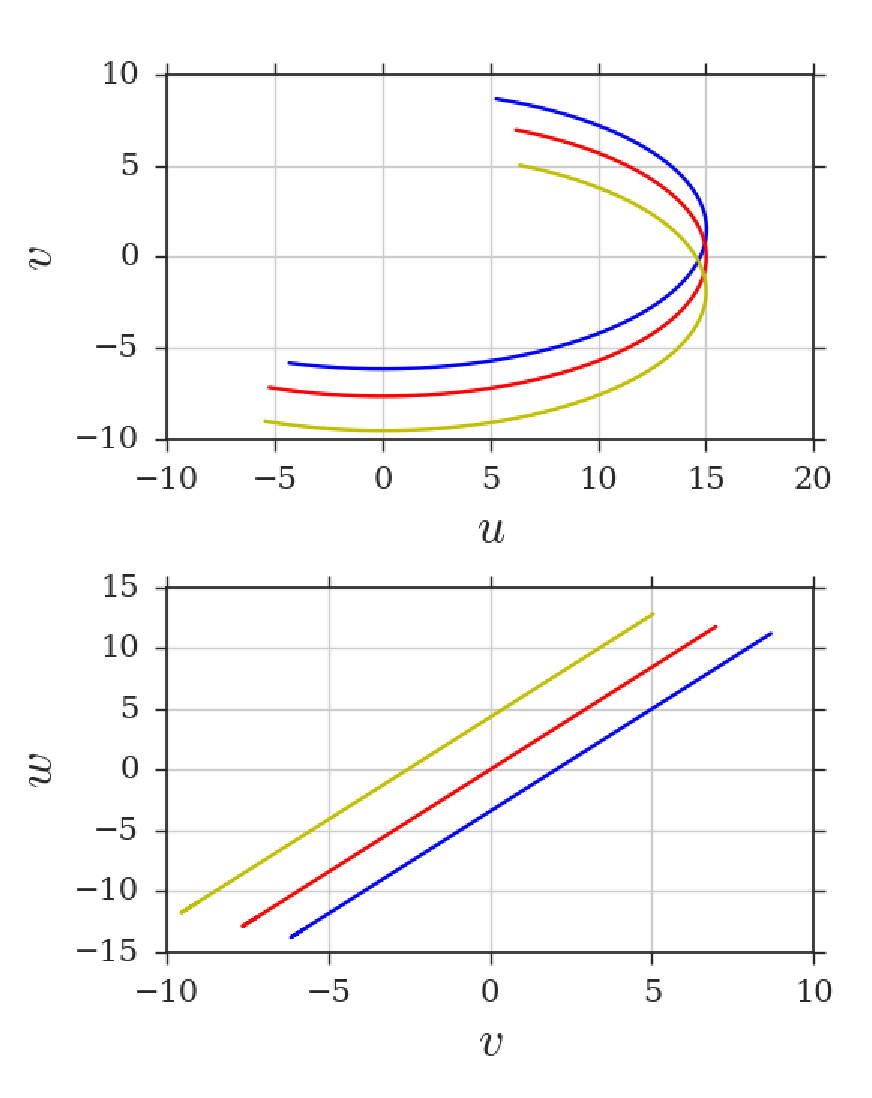
\includegraphics[width=\linewidth]{rotation_new}
\caption{Tracks of 3 PAPER-128 baseline classes shown in Fig. \ref{fig:AntPos}, here with the same respective colors. Tracks are traced out over half a sidereal day for frequency $\nu=0.15\text{GHz}$ and a phase center that passes through zenith. The top panel shows $uv$ tracks with crossings among each pair of baseline classes. Projection to the $vw$ plane in the bottom panel shows that tracks in $uvw$ space do not cross. }
\label{fig:Tracks}
\end{figure}

Equivalent baselines follow identical $uvw$ tracks. Traditionally, we can identify
redundancy of nearly equivalent baselines as crossings
of the $uv$ tracks, a 2 dimensional projection of Fig. \ref{fig:Tracks}. As we see in the top panel of Fig. \ref{fig:Tracks}, there would be many such crossings. However, there are several reasons that $uv$ track-crossing do not imply perfect redundancy. In fact, in our case $uv$ track-crossings are
not accurate enough for time offset determination, nor can it give estimate of the degree of redundancy.  The most obvious reason is that the 3 dimensional $uvw$ tracks do not actually cross, as is evident from the $vw$ projection in the bottom panel of Fig. \ref{fig:Tracks}. For drift-scan arrays, even a hypothetical crossing in $uvw$ space would not imply perfect redundancy. This shall become evident in the next section, after we develop a more general formalism that accounts for the point spread function of the finite beams, and estimate the degree of redundancy for general combination of baselines at a general time-offset. Then, relation of track-crossing and redundancy for both drift-scan and tracking measurements will be explored in Appendix \ref{sec:appA}. 



\subsection{Formalism}
In this section we formulate the relation between 
the product of delay-transformed visibilities from two arbitrary baselines and the power spectrum. 

We begin with the visibility as commonly defined in the literature (e.g.
\citealt{TMS, first-paper}): 
\begin{equation}
\begin{aligned}V_{\nu}(\boldsymbol{b}) & =\int d\Omega A(\hat{\boldsymbol{s}},\nu)\phi(\nu)I_{\nu}(\hat{\boldsymbol{s}})\exp\left(-2\pi i\frac{\nu}{c}\boldsymbol{b}\cdot\hat{\boldsymbol{s}}\right),\\
 & \approx\frac{2k_{B}}{\lambda^{2}}\int d\Omega A(\hat{\boldsymbol{s}},\nu)\phi(\nu)T(\hat{\boldsymbol{s}})\exp\left(-2\pi i\frac{\nu}{c}\boldsymbol{b}\cdot\hat{\boldsymbol{s}}\right),
\end{aligned}
\label{eq:Vis1}
\end{equation}
where $k_B$ is Boltzmann's constant, $\lambda$ is the mean wavelength, $\hat{\boldsymbol{s}}$ and $\Omega$ are a direction in the
sky and its corresponding solid angle. Inside the integral we have $\phi(\nu)$ the frequency bandpass profile, $A(\hat{\boldsymbol{s}},\nu)$ the (frequency-dependent) primary beam, and $I$ the specific intensity, which has been
related to $T$, the brightness temperature in the Rayleigh-Jeans
limit. The beam power pattern $A$ is dimensionless,
normalized to 1 at its peak (zenith), and we assume it to be the same
for all baselines. %We show sample beams of HERA and PAPER antennas in Fig. \ref{fig:Beam} for reference. 



%\begin{figure}[H]
%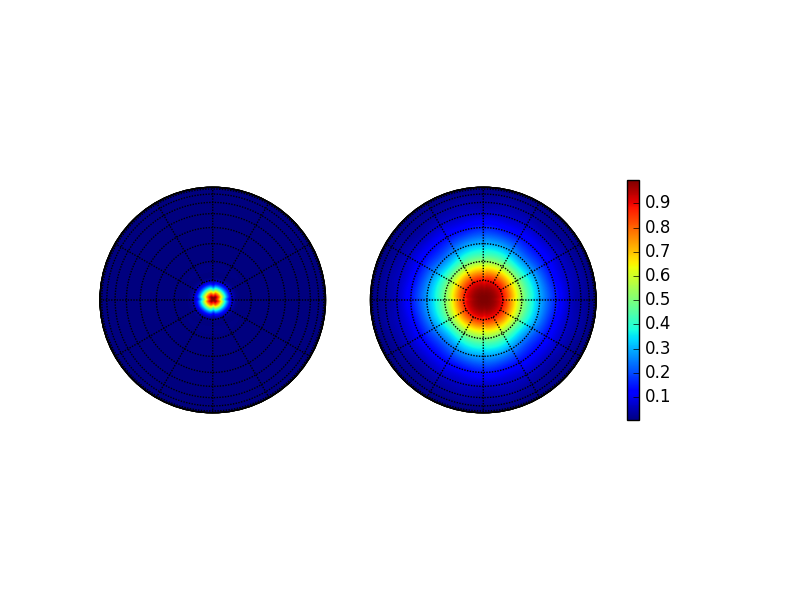
\includegraphics[width=1.2\linewidth]{Beams}

%\caption{Example beam response of HERA (left) and PAPER (right) antennas. Both beams are Stokes $I$ polarization antenna voltage beams, at frequency of $\nu=150\text{MHz}$ and normalized to $1$ at zenith. The circles centered around zenith (center of beam) here are
%spaced 10 degrees apart. \label{fig:Beam}}
%\end{figure}

Power-spectrum measurements are typically taken from $\sim10$MHz centered around the corresponding redshift of interest (e.g. 150 MHz for z=9.5). 

Delayed-transformed visibility has gained popularity in recent years since it has been shown that foregrounds are isolated in delay space. We define the delay-transformed visibility by Fourier transforming visibility along the frequency axis \citep{delay-transform} as:
\small
\begin{equation}
\begin{aligned}V(\boldsymbol{b},\tau) & =\int d\nu V_{\nu}(\boldsymbol{b})\phi(\nu)\exp\left(2\pi i\nu\tau\right),\\
 & =\frac{2k_{B}}{\lambda^{2}}\int d\Omega d\nu A(\hat{\boldsymbol{s}},\nu)T(\hat{\boldsymbol{s}},\nu)\exp\left[-2\pi i\nu\left(\frac{\boldsymbol{b}\cdot\hat{\boldsymbol{s}}}{c}-\tau\right)\right]. 
\end{aligned}
\label{eq:Vb1}
\end{equation}
\normalsize
Here the delay $\tau$ is the Fourier dual of $\nu$. Eq. \eqref{eq:Vb1} expresses the delay-transformed visibility as
an integral over observational coordinates $\hat{\boldsymbol{s}}$ and $\nu$. For notational simplicity here and in the rest of this paper, we shall absorb the bandpass $\phi$ inside the primary beam $A$.  

Ultimately,
we would like to relate the data, collected with coordinates $\hat{\boldsymbol{s}}$
and $\nu$, to the power spectrum, written with 
$\boldsymbol{r}$ and $\boldsymbol{k}$, the cosmological position coordinate and wavenumber. To do so, we start by noticing that
\[
\begin{aligned}r & =\frac{c}{H_{0}}\int_{0}^{z}\frac{dz'}{E(z')},\\
 & \approx\frac{c}{H_{0}}\int_{0}^{z_{0}}\frac{dz'}{E(z')}-\frac{c(1+z)^{2}}{\nu_{21}H_{0}E(z)}\left(\nu-\nu_{0}\right),\\
 & \equiv X-Y\Delta\nu,
\end{aligned} \label{eq:r}
\]
where $\nu_{21}=1420$MHz is the 21\,cm transition rest frequency, $\nu_{0}$
a reference central frequency with corresponding redshift $z_{0}$,
and 
\[
E(z)=\sqrt{\Omega_{m}(1+z)^{3}+\Omega_{\Lambda}}.
\]
Inverting for $\nu$:
\begin{equation}
\nu=\frac{X-r}{Y}+\nu_{21}.\label{eq:nur}
\end{equation}

In the thin-shell limit, we can write:
\begin{equation}
d^2r=X^2d\Omega. 
\label{eq:thinshell}
\end{equation}
Note Eq. \eqref{eq:thinshell} does not require the flat-sky approximation; the angular integral is still performed over the curved sky. 

We can rewrite the delayed-transformed visibility as 
\small
\[
\begin{aligned}V(\boldsymbol{b},\tau) & =\frac{2k_{B}}{\lambda^{2}}\int\frac{d^{3}r}{X^{2}Y}A(\boldsymbol{r})T(\boldsymbol{r})\exp\left[-2\pi i\left(\frac{\boldsymbol{b}}{c}\cdot\hat{\boldsymbol{r}}-\tau\right)\nu_{r}\right],
\end{aligned}
\]
\normalsize
 where $d\nu=-dr/Y$ and $d^{3}r=-X^{2}Yd\Omega d\nu$. 
We have written $\nu_{r}$ as a reminder that $\nu$ and $r$ are related
by Eq. \eqref{eq:nur}. 

Existing visibility based power-spectrum pipelines for redundant drift-scan  arrays relate the power-spectrum to the conjugate square of the visibilities \citep{delay-transform, paper32, Ali2015}. We would like to generalize such relations by relating the power-spectrum to the product of two visibilities from two arbitrary baselines and time-offsets. 
The beam pattern of a baseline shifts relative to the sky as the Earth rotates. Here we choose to fix the sky, and denote the rotated coordinates
in the topocentric frame with the 3 dimensional rotation operator $\Gamma$:

\[
\begin{aligned}V_{\psi}(\boldsymbol{b'},\tau) & =\frac{2k_{B}}{\lambda^{2}}\int\frac{d^{3}r}{X^{2}Y}A(\Gamma\boldsymbol{r})T(\boldsymbol{r})\\
& \qquad \qquad  \exp\left[-2\pi i\left(\frac{\boldsymbol{b}}{c}\cdot\Gamma\hat{\boldsymbol{r}}-\tau\right)\nu_{r}-i\psi_\nu\right],\end{aligned}
\]
where we introduced a frequency-dependent phase $\psi_{\nu}$, which to first order corresponds to phasing the two visibilities to the same phase center. \footnote{Turns out for many cases, the first-order interpretation is largely sufficient, but we still keep the term to reserve the option to determine its exact form numerically. } 

With implicit bounds of integrals from $-\infty$ to $\infty$, we have:
\begin{widetext}
\begin{equation}
\begin{aligned} & \langle V^{*}(\boldsymbol{b},\tau)V_{\psi}(\boldsymbol{b'},\tau)\rangle\\
 & =\left(\frac{2k_{B}}{X^{2}Y\lambda^{2}}\right)^{2}\int d^{3}rd^{3}r'\left(\langle T^{*}(\boldsymbol{r})T(\boldsymbol{r'})\rangle\right)A^{*}(\boldsymbol{r})A(\Gamma \boldsymbol{r'})\Phi_{b,\tau}(\boldsymbol{r},\Gamma \boldsymbol{r'}),\\
 & =\left(\frac{2k_{B}}{X^{2}Y\lambda^{2}}\right)^{2}\int d^{3}rd^{3}r'\left(\int\frac{d^{3}\kappa}{(2\pi)^{3}}\frac{d^{3}\kappa'}{(2\pi)^{3}}\langle T^{*}(\boldsymbol{\kappa})T(\boldsymbol{\kappa'})\rangle e^{-i(\boldsymbol{\kappa}\cdot \boldsymbol{r}-\boldsymbol{\kappa'}\cdot\boldsymbol{r'})}\right)A^{*}(\boldsymbol{r})A(\Gamma \boldsymbol{r'})\Phi_{b,\tau}(\boldsymbol{r},\Gamma \boldsymbol{r'}),\\
 & =\left(\frac{2k_{B}}{X^{2}Y\lambda^{2}}\right)^{2}\int d^{3}rd^{3}r'\left(\int\frac{d^{3}\kappa}{(2\pi)^{3}}P(\kappa)e^{-i\boldsymbol{\kappa}\cdot(\boldsymbol{r}-\boldsymbol{r'})}\right)A^{*}(\boldsymbol{r})A(\Gamma \boldsymbol{r'})\Phi_{b,\tau}(\boldsymbol{r},\Gamma \boldsymbol{r'}),\\
 & \approx\left(\frac{2k_{B}}{X^{2}Y\lambda^{2}}\right)^{2}P(k_{b,\tau})\int d^{3}rd^{3}r'\delta_{D}^{(3)}(\boldsymbol{r}-\boldsymbol{r'})A^{*}(\boldsymbol{r})A(\Gamma \boldsymbol{r'})\Phi_{b,\tau}(\boldsymbol{r},\Gamma \boldsymbol{r'}),\\
 & =\left(\frac{2k_{B}}{X^{2}Y\lambda^{2}}\right)^{2}P(k_{b,\tau})\int d^{3}rA^{*}(\boldsymbol{r})A(\Gamma \boldsymbol{r})\exp\left[-i2\pi\frac{\nu_{r}}{c}\left(\hat{\boldsymbol{r}}\cdot\boldsymbol{b}-\Gamma \hat{\boldsymbol{r}}\cdot\boldsymbol{b'}\right)-i\psi_{\nu}\right],\\
 & =\left(\frac{2k_{B}}{\lambda^{2}}\right)^{2}P(k_{b,\tau})\int\frac{d\Omega d\nu}{X^{2}Y}A^{*}(\hat{\boldsymbol{s}},\nu)A(\Gamma \hat{\boldsymbol{s}},\nu)\exp\left[-i2\pi\frac{\nu}{c}\left(\hat{\boldsymbol{s}}\cdot\boldsymbol{b}-\Gamma\hat{\boldsymbol{s}}\cdot\boldsymbol{b'}\right)-i\psi_{\nu}\right],
\end{aligned}
\label{eq:main}
\end{equation}
In transition from cosmological coordinates back to observing coordinates we have written $\hat{\boldsymbol{r}}\equiv\hat{\boldsymbol{s}}$, and 
\begin{equation}
\Phi_{b,\tau}(\boldsymbol{r},\Gamma \boldsymbol{r'})\equiv\exp\left[i\frac{2\pi}{c}\left(\boldsymbol{b}\cdot\nu_{r}\hat{\boldsymbol{r}}-\boldsymbol{b'}\cdot\nu_{r'}\Gamma\hat{\boldsymbol{r'}}\right)\right]\exp\left[-i2\pi\tau\left(\nu_{r}-\nu_{r'}\right)-i\psi_{\nu}\right].
\end{equation}
\end{widetext}
The third equality of Eq.(\ref{eq:main}) follows from assumption of translational invariance of statistics of the 21\,cm field, and the first inequality follows from the assumption that
the 3D power spectrum varies negligibly over the $k$-space of interest. The careful reader may have noticed that we have also assumed here a definitive relation between $k$ and $b,\tau$. In the flat-sky limit for example, such a relation would take the form $(Xk_{x},Xk_{y},Yk_{z})=\frac{2\pi}{c}(b_{x},b_{y},\tau)$. Instrumental chromaticity and foreground isolation will be examined in \ref{sec:chromaticity}. Since $\Gamma$
is a sky rotation, it does not affect $\nu$, hence we have taken $\nu_{r}$
outside the parenthesis in the phase term $\exp\left[-i2\pi\frac{\nu_{r}}{c}\left(\hat{\boldsymbol{r}}\cdot\boldsymbol{b}-\Gamma \hat{\boldsymbol{r}}\cdot\boldsymbol{b'}\right)\right]$. Notice that the phase factor $\exp\left[-i2\pi\tau\left(\nu-\nu'\right)\right]$
drops out in the end. This means that the location and magnitude of the correlation peak does not depend on delay $\tau$. 

Since the beam pattern and bandwidth are given in $\hat{\boldsymbol{s}}$
and $\nu$, we convert the integral back to these coordinates to get
the general relation between the delay-transformed visibilities and
the power spectrum:

\begin{equation}
\begin{aligned} & \langle V^{*}(\boldsymbol{b},\tau)V_{\psi}(\boldsymbol{b'},\tau)\rangle\\
 & =\left(\frac{2k_{B}}{\lambda^{2}}\right)^{2}P(k_{b,\tau})\int\frac{d\Omega d\nu}{X^{2}Y}A^{*}(\hat{\boldsymbol{s}},\nu)A(\Gamma\hat{\boldsymbol{s}},\nu)\\
 & \qquad \qquad \qquad \qquad \exp\left[i2\pi\frac{\nu}{c}\left(\hat{\boldsymbol{s}}\cdot\boldsymbol{b}-\Gamma\hat{\boldsymbol{s}}\cdot\boldsymbol{b'}\right)-i\psi_{\nu}\right].
 \end{aligned}
\label{eq:final}
\end{equation}

In other words the power spectrum estimate from visibilities of a baseline pair is given by 
\begin{equation}
 \hat{P}(k_{b,\tau}) \equiv \left(\frac{\lambda^{2}}{2k_{B}}\right)^{2} \frac{V^{*}(\boldsymbol{b},\tau)V_{\psi}(\boldsymbol{b'},\tau)}{\Theta}, 
 \label{eq:opp}
\end{equation}
where the weight is defined as 
\begin{equation}
\Theta \equiv\int d\nu \Theta_{\nu}, 
\label{eq:Theta}
\end{equation}
with  

\[
\Theta_{\nu} \equiv \int \frac{d\Omega}{X^{2}Y}A^{*}(\hat{\boldsymbol{s}},\nu)A(\Gamma\hat{\boldsymbol{s}},\nu) e^{i2\pi\frac{\nu}{c}\left(\hat{\boldsymbol{s}}\cdot\boldsymbol{b}-\Gamma\hat{\boldsymbol{s}}\cdot\boldsymbol{b'}\right)}e^{-i\psi_{\nu}}.
\label{eq:Thetanu}
\]


Notice that $\Theta$ has no dependence on $\tau$. In Eq. \eqref{eq:Thetanu} we introduced an extra phase $\psi$, the origin of which we shall explain in \ref{sec:rephs}. We point out that although all our derivations focused on drift-scan telescopes, we can get the analogous result for tracking measurements simply by noticing that for a tracking primary beam, $\Gamma$ becomes a rotation around zenith, and so:
\[
\Theta_{\nu} \equiv \int \frac{d\Omega}{X^{2}Y}A^{*}(\hat{\boldsymbol{s}},\nu)A(\hat{\boldsymbol{s}},\nu) e^{i2\pi\frac{\nu}{c}\left(\hat{\boldsymbol{s}}\cdot\boldsymbol{b}-\Gamma\hat{\boldsymbol{s}}\cdot\boldsymbol{b'}\right)}e^{-i\psi_{\nu}}.
\label{eq:Thetanu_tracking}
\]

Roughly speaking, Eqs. \eqref{eq:opp} through \eqref{eq:Thetanu} tell us that the cross multiplications of visibilities at a time delay is proportional to the power spectrum times the Fourier
transform of the cross multiplied beam patterns. As a check, when applied to equivalent baselines,
$\boldsymbol{b}=\boldsymbol{b'}$, $\hat{\boldsymbol{s}}=\Gamma\hat{\boldsymbol{s}}$, and Eq.(\ref{eq:final}) reduces to Eq.(B9) of \cite{paper32}. 
With Eq. \eqref{eq:opp} and Eq. \eqref{eq:Theta} we can, for any given pair of baseline classes and time delay, estimate the degree of redundancy, here represented by $\Theta$. This allows us to achieve our goals stated in the introduction: to identify 
candidate baseline pairs with significant redundancy, to find the time offset that maximizes redundancy, and to quantify the degree of such redundancy. We can do all the above simply by computing the weight $\Theta$ from
Eq.(\ref{eq:Theta}) for various time offsets. 



\subsection{Rephasing \label{sec:rephs}}
If $\psi_{\nu}=0$ in  Eq. \eqref{eq:Thetanu}, $\Theta_{\nu}$ at the peak of correlation is in general complex, and often far from real. Furthermore, this phase of peak correlation is inevitably frequency dependent. This frequency dependence of the phase would lead to destructive interference when we integrate over frequency, unless we correct $\Theta_{\nu}$ by an extra phase $\psi_\nu$. 

To first order, the physical origin of $\psi_\nu$ lies in the two visibilities having different phase centers. By default the correlators of a drift-scan array phase the two visibilities both to zenith at the same time. When they are cross-multiplied with a time lag, the visibilities must be rephased before delay transform to the account for the movement of the zenith. The effect of the phase thus roughly corresponds in a shift of the delay mode measured, and we should expect $\psi_{\nu}$ to be in first order a linear function of $\nu$:
\[
\psi_{\nu}\sim 2\pi\Delta\tau\nu.
\]
In Fig. \ref{fig:phi_nu} we show the peak phases for for a given baseline pair of PAPER128 (\{2,0\}:\{2,1\}), comparing the drift-scan phase dependence with that of the same baseline with hypothetical tracking-elements (Eq. \eqref{eq:Thetanu} and Eq. \eqref{eq:Thetanu_tracking}). In the drift-scan case, we indeed see a linear relation corresponding to a delay of $\Delta\tau\approx15.7$ns. In the tracking case, because of minimal zenith movement, only second order effects are observed. The origin of the second order effects can be seen as due to the $w$-term, or more precisely the fact that $uvw$ tracks do not cross when their 2 dimensional projections do. We refer the reader to Appendix \ref{sec:appA} for further explanation. In both cases, the full effects are encapsulated in the phase of $\Theta_\nu$ and can be thus determined empirically without any additional computation. 

\begin{figure}[H]
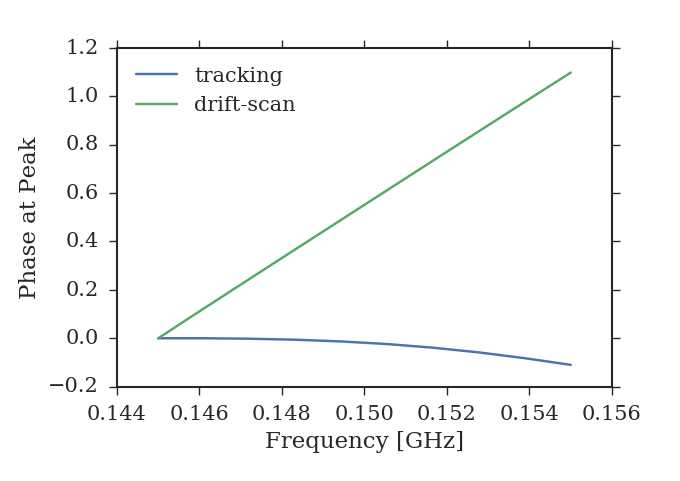
\includegraphics[width=1\linewidth]{phi_nu}

\caption{Frequency dependent peak phases for PAPER-128 baseline pair \{2,0\}:\{2,1\}. Both the drift-scan case and a hypothetical tracking baseline are shown in solid lines. The first-order, linear effects are shown in dashed lines. We have also fixed the global phase in both cases to 0 at 0.15GHz. The drift-scan case exhibits linear behavior and conforms well to the first order effect of a shift in delay space due to the movement of zenith. }
\label{fig:phi_nu}
\end{figure}


To illustrate the effect of rephasing, we compare in Fig. \ref{fig:freqdiff} real parts of $\Theta_{\nu}$ of both equivalent and nearly equivalent baseline pairs for two channels: 0.145 GHz and 0.155 GHz. The top two panels have zero rephasing, and the bottom two are linearly rephased to a differential delay of $\Delta\tau\approx15.7$ns, as we determined above. The first and third panels show the equivalent baseline pairs \{2,0\}:\{2,0\}, and second and fourth panels show \{2,0\}:\{2,1\}. Summing over frequency without proper rephasing leads to destructive interference and signal loss. The wider the frequency profile, the more destructive the interference would be. Only after rephasing to the correct time-offset for each baseline pairs can we constructively combine the frequency channels. 

We see from Fig. \ref{fig:freqdiff} that although the amplitude of correlations match up for all time offsets, the phase would only locally match. The need for rephasing can thus be understood as a symptom of the underlying spatial decoherence; coherence at the phase center would not extend to the entire beam pattern (Fig. \ref{fig:beamfringe}). Thus while integrating over frequencies and sky-direction in Eq. \eqref{eq:Theta} there are necessarily sky-directions that do not add coherently. This decoherence across the beam pattern cannot be removed and plays a fundamental role in determining how much sensitivity one can recover from nearly equivalent baselines. 

\begin{figure}[H]
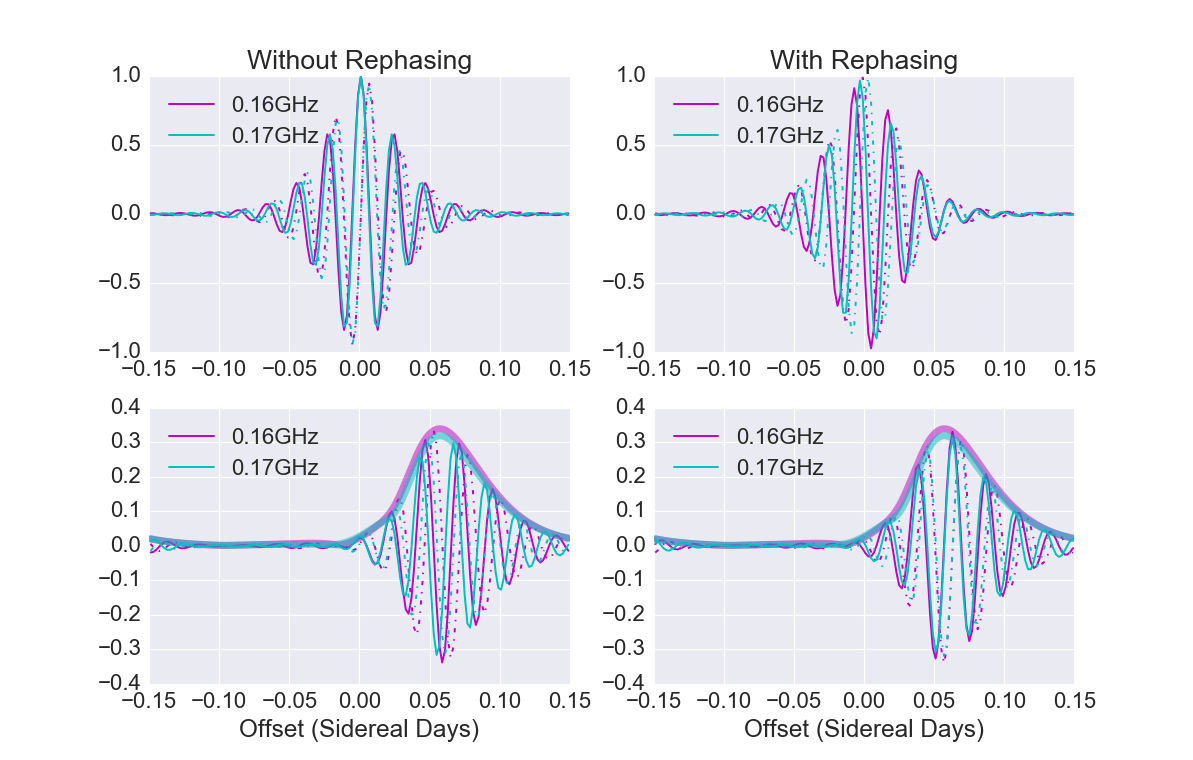
\includegraphics[width=1.1\linewidth]{rephs}

\caption{Comparisons of the peak phases of two different frequencies. Specifically shown are the real parts of $\Theta_{\nu}$. First and third panels shows equivalent baselines, second and fourth show a pair of nearly equivalents. The top two panels have zero phase shift ($\psi_{\nu}=0$), and the bottom two are rephased to a time offset of 0.0325 sidereal days. The first and last panels thus show a coherently rephased series that would add constructively at the respective peaks. }
\label{fig:freqdiff}
\end{figure}

\section{Analysis}

In this section we delve into visualizing and testing our method, and explore sensitivity contributions of various baseline classes for PAPER and HERA array configurations. 
\subsection{Visualization \label{sec:visual}}

So far for clarity and generality we have avoided the traditional formulation of radio astronomy in terms of the $uv$-plane. To gain some visual intuition of the formalism in Section \ref{sec:method}, we show explicit beam fringe patterns of the two baselines and their interactions. For this section, we relax into the flat sky approximation so that $(l,m,\sqrt{1-l^2-m^2})\equiv\hat{s}$ and examine a single frequency of $150$MHz. 

At the time-offset of maximum redundancy, we expect two beams to have to same fringe pattern in both frequency and phase. Due to the time delay, however, the beam centers would be slightly shifted with respect to each other. This we show in the top panels of Fig. \ref{fig:beamfringe}. The top left and middle panels show the beam-fringe
patterns (real parts) for baselines \{2,0\} and \{2,1\}, delayed by 0.0325 sidereal days.
The product of the beam fringe patterns in top right shows that the fringes
 cancel out as we expect. On the bottom of Fig. \ref{fig:beamfringe} we show the instantaneous $uv$ coverage of two baselines and their product. We see from the bottom right panel that the cross-multiplied baselines recover  power concentrated at $u\approx\frac{30\text{m}}{c/1.5\times10^8\text{Hz}}\approx15$. Note the bottom right panel is not the Fourier transform of the top right panel. 

\begin{figure*}[h!]
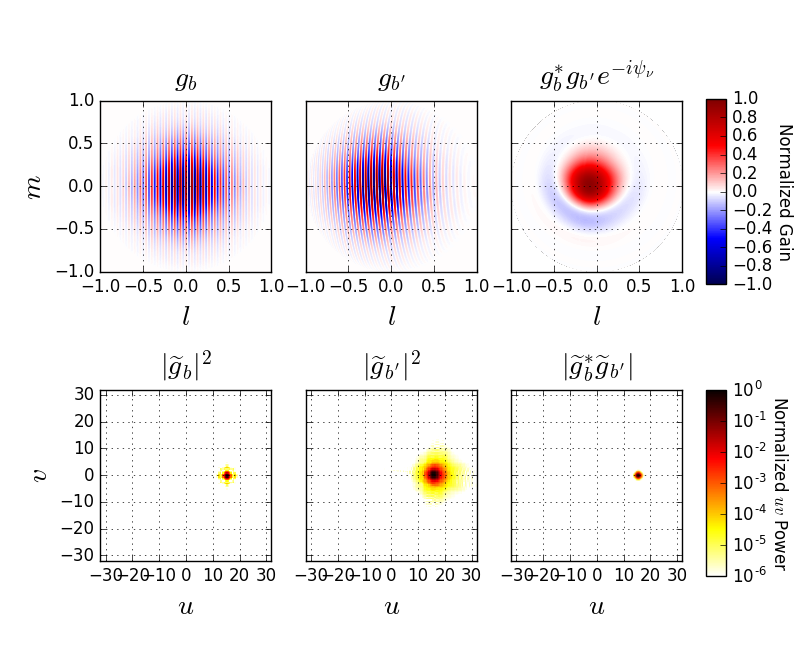
\includegraphics[width=\textwidth]{BeamFringe}

\caption{PAPER128 beam-fringe patterns and their point-spread functions on the $uv$-plane for a frequency of $150$MHz. Selected baselines have 30 meter East-West separation, and 0 and 4 meter North-South separation, respectively. The top panels show the real parts of the beam-fringe patterns of the baselines (left and middle), and their conjugate product (right). The beam-fringe values are normalized such that the peak of the original beam is unity. 
The bottom left and middle panels show the peak-normalized $uv$ beam power of the two beam-fringe patterns. The product of the beam spreads displayed in the bottom right panel shows that power concentrated at $u\approx15$ is recovered. }
\label{fig:beamfringe}
\end{figure*}


\subsection{Numerical Test \label{sec:Techniquet}}

Bringing together the discussion from Section \ref{sec:method}, we present a numerical check of Eq. \eqref{eq:final}, including rephasing. To do so, we need to compare the amplitude and phase of the integral weight $\Theta$ 
for a pair of baselines with products of simulated visibilities of those baselines. We use 10 frequency channels evenly spaced from $145$MHz to $155$MHz for the comparison. We rephase one of the simulated visibilities, as well as computed $\Theta_{\nu}$ to the same delay as computed from the peak phase of the latter. 
 
\begin{figure}[h]
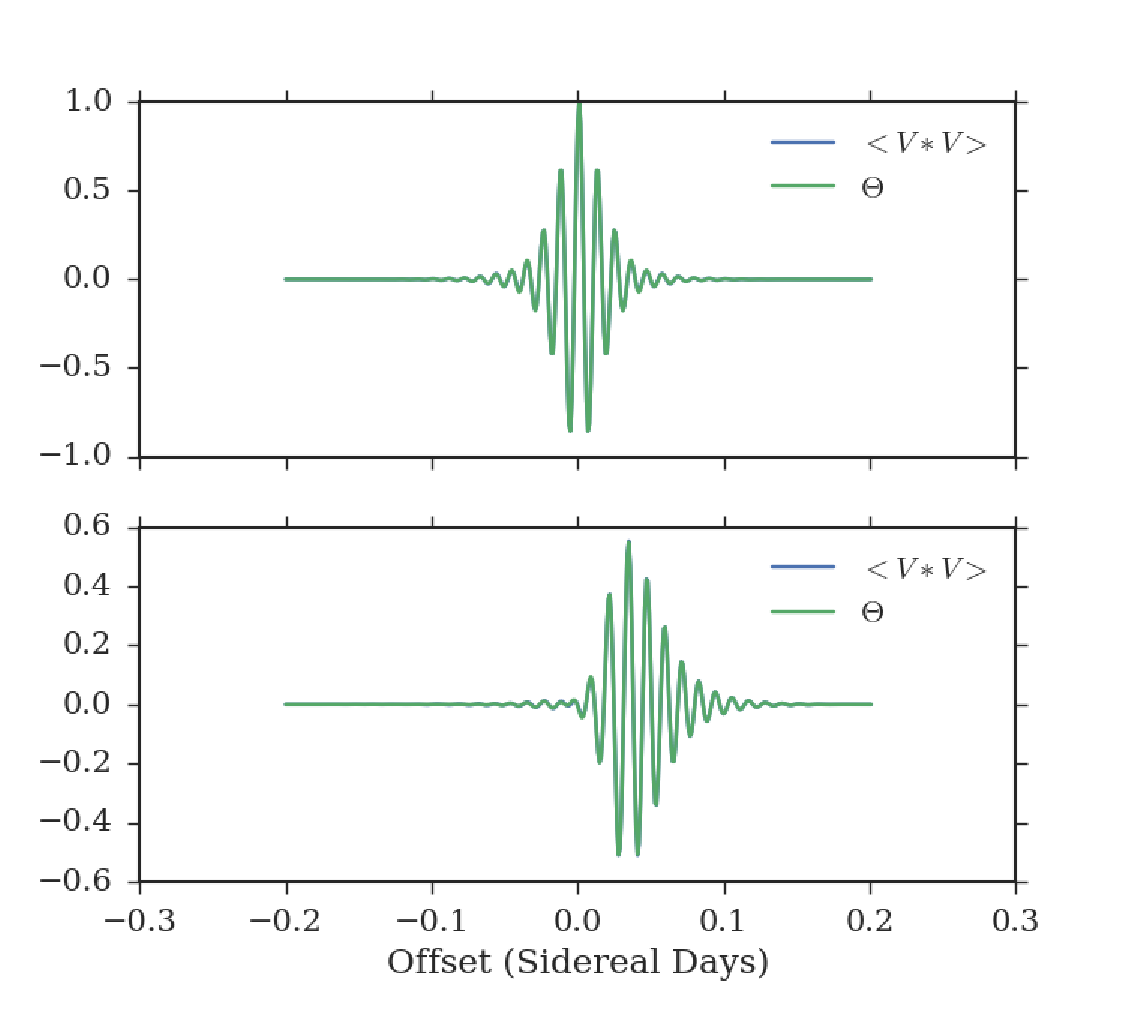
\includegraphics[width=\linewidth]{numerics}

\caption{Numerical comparisons of the visibility correlation peaks to the $\Omega$ factor in Eq.(\ref{eq:final}). We generated a Gaussian random sky on healpix maps, computed visibilities and cross correlated them to find the correlation.  Top panel shows the equivalent baseline pairs \{2,0\} against \{2,0\}, bottom panel shows \{2,0\} against \{2,1\}.  Evaluations of weight $\Theta$ are shown green, and the visibility correlations of simulated random sky is given in blue. In both cases only the real parts are shown. We see that in both cases the theory and simulation line up in both amplitude and phase.}
\label{fig:numerics}
\end{figure}

Fig. \ref{fig:numerics} shows the real parts of the resulting degree of redundancy as a function of time offset, for equivalent baseline pairs (\{2,0\}:\{2,0\}) in the top panel and nearly equivalent (\{2,0\}:\{2,1\}) in the bottom. Shown in green for the two cases are the computed values of $\Theta$, both normalized to the peak of the equivalent case. The plot on the bottom is rephased with a delay of $\Delta\tau\approx15.7$ns as outlined in Section \ref{sec:rephs}. Since both y-axes are normalized to the same scale, we see the equivalent baseline reach maximal redundancy with 0 time-offset, while the nearly equivalent pair reaches maximum redundancy of $\Theta\approx0.5$ at $dT\approx0.325$days. 

Almost completely overlapping with the green curves are the cross-multiplied visibilities from a simple simulation, shown in blue. For the simulation, we populate random values of brightness temperature
on a healpix map \citep{Heal, HealPrimer} \footnote{We use functionalities in the python package AIPY for healpix mapping
as well as coordinate transforms. }. We rotate the baseline positions with
the appropriate rotation matrix, multiplying the sky by the primary beam to get the visibilities, for each
baseline\footnote{There are two obvious ways to achieve the rotation. One
can either fix the sky and rotate the baselines, or the other way
around. We found however, that we must not physically rotate the sky
map, for the numerical round-offs due to finite resolutions of the
map turns out to be significant. Thus we let the sky, represented
by the healpix map, be fixed, and rotate the baselines. }. For the nearly equivalent case, we rephase the delayed visibility (\{2,0\}) by the same delay $\Delta\tau\approx17$ns, followed by delay-transform. The resulting delay-space visibilities for the two baselines are then convolved
via the Fourier convolution theorem, to obtain values of the cross
correlation as a function of time-offset.   We do this for both the equivalent (\{2,0\}:\{2,0\}) and nearly equivalent (\{2,0\}:\{2,1\}) case.
Since the blue and green curves overlap, we have verified that in this case Eq. \eqref{eq:final} is valid and the computed $\Theta$ can be used as weight to obtain the power spectrum. 


\subsection{Chromaticity \label{sec:chromaticity}}
Manageable chromaticity of the instrument is crucial in delay-transform technique of foreground isolation. Previous studies have shown that smooth foreground are constrainted in a "wedge" structure in cosmological $k$ space \citep{wedge1, wedge2}. We must show that our method does not destroy the ability of delay-transform to isolate foreground.[ ..... ]










\begin{figure*}[h!]
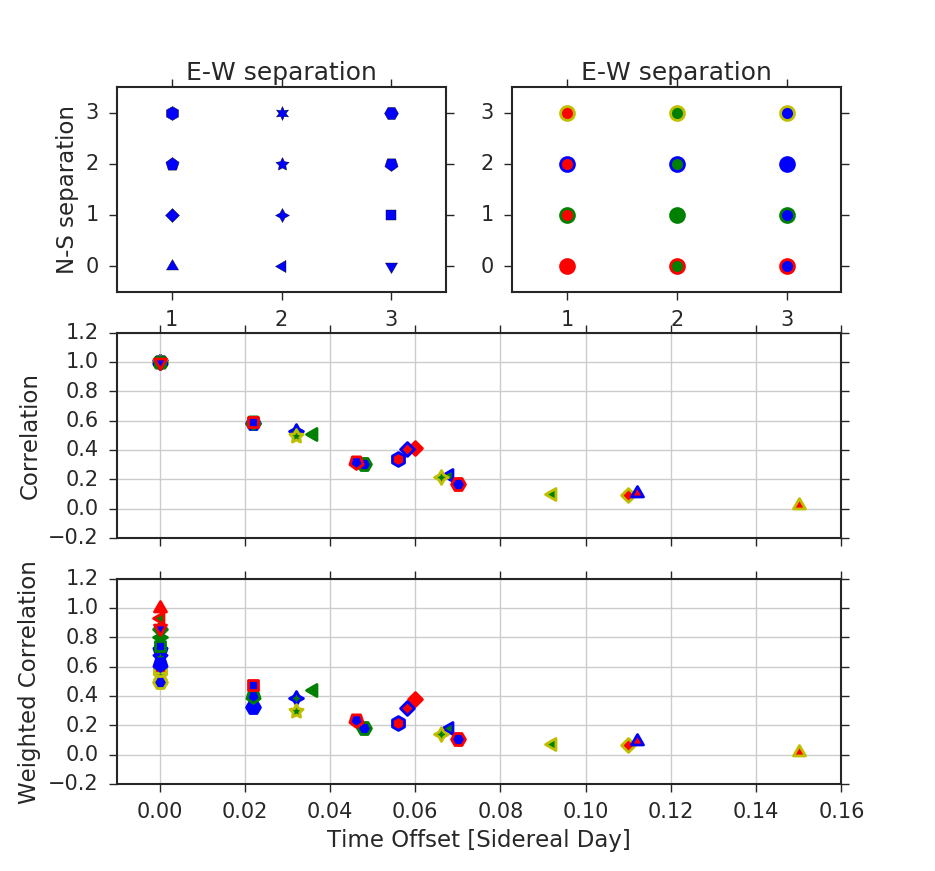
\includegraphics[width=0.95\textwidth]{sensitivity_1}

\caption{Relative sensitivity contributions of selected baseline combinations in PAPER-128. Each labeled point in the middle and bottom panels correspond to a cross-correlated baseline pair \{m,n\}:\{p,q\}. The shape of the symbol encodes the first baseline \{m,n\}, as displayed in the top left legend panel. The edge and face colors encode the second baseline \{p,q\}, as displayed in the top right legend panel. The middle
panel shows the peak height ($\Theta$) of each baseline
combination, while the bottom panel multiplies the heights by the
corresponding multiplicities as in Eq. \eqref{eq:sensul}. 
In both the middle and bottom panels, we have chosen to fix the value  of \{1,0\}:\{1,0\} to unity.  }
\label{fig:sensplot}
\end{figure*}

\begin{figure}[h]
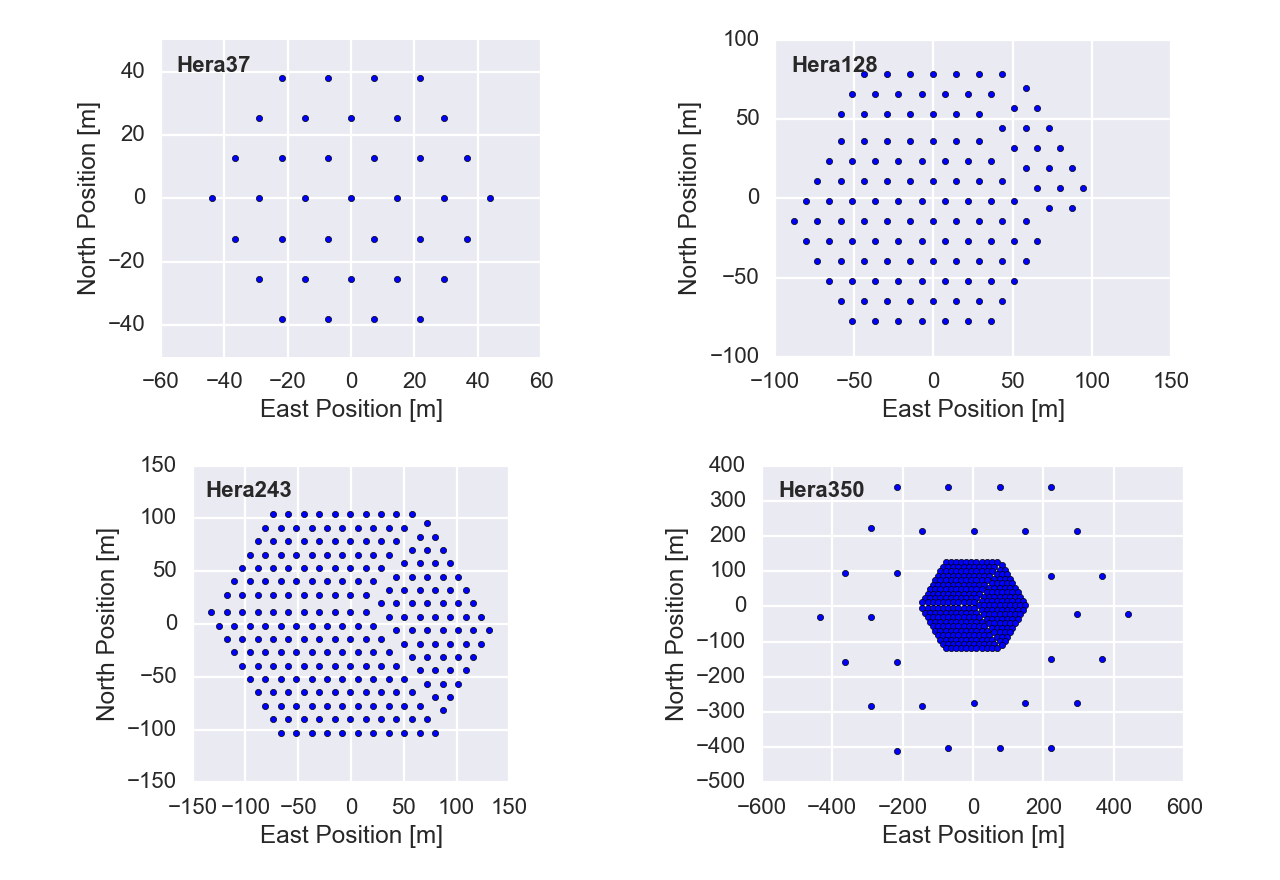
\includegraphics[width=\linewidth]{HeraAntpos}
\label{fig:HeraAntpos}
\caption{Planned Hydrogen Epoch of Reionization Array antenna configurations. HERA 37 is expected to complete and start collecting data in summer of 2017, and the other three are planned configurations in the next phases. For HERA350, only the 320 elements in the core are shown. }
\end{figure}

\subsection{ Sensitivity \label{sec:sensitivity}}
In this section we discuss the sensitivity contributions of a variety of baseline pairs from PAPER128.
Recall the sensitivity contributions of a particular baseline pair is given by $\Theta$ (Eq. \eqref{eq:Theta}). 
%Intuitively we expect the sensitivity to depend on both the $uv$ coverage of the baseline and the patch of sky inside the beam. A larger beam like that of PAPER would tolerate larger time-offsets because more sky area can coincide in the two beams \footnote{Larger beams also imply smaller spread in $uv$ space. This could lead to either larger or smaller redundancy, which depends on the overlap of two such point spread functions.}


In the middle panel of Fig. \ref{fig:sensplot}
we show the peak heights $\Theta$ and locations $\Delta T$ for a variety of baseline combinations. Baseline pairs that are mirror images of each other 
give the same amount of redundancies ($\Theta$), with the opposite time offset, as expected from symmetry. 
For example, \{1,0\}:\{1,1\} is mirror image of \{1,0\}:\{1,-1\} and these two pairs of baselines
give the same sensibility contribution. Thus we only show a subset of representative baseline pairs to illustrate the contributions. For a more complete result see Fig. \ref{fig:pairplot}.  

Baseline pairs that have smaller optimal time delays
tend to have higher correlations. In other words, correlation peaks
that are closer to zero time offset are higher. This is expected for two reasons;
number one is that the longer the time delay that produces redundancy, the more the sky has moved with respect
to the beams and hence the less overlaps in patch of sky surveyed. The other reason is that smaller optimal
time-offset corresponds to smaller differences in orientation and length of the pair of baselines and hence better redundancy. 


To determine that actual relative contribution to sensitivity of these
baseline pairs, we have to account for the multiplicities of
these baseline classes, in other words the number of antenna pairs with the
same length and orientation. We would like to estimate an effective weight $\widetilde{\Theta}$ that accounts for both the peak height $\Theta$ and the multiplicities of the baseline classes. From Fig. \ref{fig:sensplot}
we see for example \{1,0\} has higher multiplicity than \{2,0\},
or \{1,1\}. The latest release of PAPER64 data uses the PAPER128-equivalent baselines \{2,1\},
\{2,0\} and \{2,-1\} \citep{Ali2015}. There, the three sets of equivalent baseline classes
are only cross multiplied with itself. Assuming that each equivalent baseline delivers
the same $\Theta$, the relative contribution to sensitivity can be estimated. 

First we can average the visibilities of the equivalent baselines. Since the core of PAPER-128 has 16 by 7 antenna configuration, there
are $M\equiv(16-|m|)\times(7-|n|)$ copies of the baseline class $\{m,n\}$. This means
that if we add visibility measurements of all the equivalent baselines,
we get a factor of $\sqrt{M}$ reduction in noise
level $\sigma_N$ of the visibility. The sensitivity contribution of $\{m,n\}$, cross multiplied with $\{m',n'\}$  thus roughly scales as $\sqrt{\left((16-|m|)(7-|n|)(16-|m'|)(7-|n'|)\right)}=\sqrt{MM'}$.
For cross-multiplications of nearly equivalent baselines of
types $\{m,n\}$ and $\{m',n'\}$, we get an effective weight: 

\begin{equation}
\widetilde{\Theta}_{bb'} \propto \Theta_{bb'}\times\sqrt{MM'}.\label{eq:sensul}
\end{equation}

Shown in the bottom panel of Fig. \ref{fig:sensplot} are the peak heights weighted
by the multiplicity factor. Points that have zero time delay are the equivalent baseline pairs and their weighted correlation values simply reflect the multiplicity factor. For clarity of presentation we have ``folded over'' the negative time delays and combined baseline pairs that are identical modulus parity. We point out that the data points shown here are not all the cases of highest correlation.  

With $\widetilde{\Theta}$, we can estimate the power spectrum by inverse covariance weighting:
\begin{equation}
\begin{aligned}
 P(k_{\tau}) &= \frac{\sum_{bb'}P(k_{b,\tau})/\sigma_P^2(bb')}{\sum_{bb'}\sigma_P^2(bb')}, \\
 &= \frac{\sum_{bb'}P(k_{b,\tau})\widetilde{\Theta}_{bb'}^2}{\sum_{bb'}\widetilde{\Theta}_{bb'}^2},
 \end{aligned}
\end{equation}
where the sum is over classes of baseline pairs. 
We define the estimator sensitivity to be the inverse of the power spectrum noise variance:
\begin{equation}
\rho \propto \frac{1}{\sigma_P^2} \propto \rho_0^2\sum_{bb'}^N\widetilde{\Theta}^2_{bb'},
\end{equation}
where, if $\sigma_S^2$ and $\sigma_N^2$ are the characteristic signal and noise levels of a single-baseline visibility, $\rho_0\equiv\sigma_S^2/\sigma_N^2$ is the signal to noise ratio. 


The scaling in Eq. \eqref{eq:sensul} was rough for simplicity of motivation. As we derive in Appendix \ref{sec:appB}, this weight should be corrected by a factor proportional $\rho_0$:

\begin{equation}
\label{eq:tildereal}
\widetilde{\Theta}_{bb'}=\frac{\Theta_{bb'}\sqrt{M_bM_{b'}}}{\sqrt{1 + \rho_0 \left(M_b+M_{b'} \right)}}.
\end{equation}

For a given $\rho_0$ Eq. \eqref{eq:tildereal} quantifies the relative sensitivity contribution of a baseline pair $bb'$. Assuming a reionization signal of $\Delta_{21cm}^2\sim 30mK^2$, observation centered at 150MHz ($z=8.5$), and 120 days of integration with PAPER antennas, we have roughly
(See Eq.(20) in \cite{first-paper})
\begin{equation}
\rho_0 \sim 0.001\left[\frac{L}{40m}\right] \left[\frac{0.1hMpc^{-1}}{k}\right]^3, 
\end{equation}
where $L$ is the average baseline length between the pair. As expected, baseline-pairs that have smaller $\widetilde{\Theta}$ contribute less to the sensitivity. 

\subsection{Array Configuration Comparisons \label{sec:arrconf}}
We run our algorithm over all possible baseline-pairs of  PAPER128, HERA37, HERA128, HERA243 and HERA350. The HERA antenna configurations are shown in Fig. \ref{fig:HeraAntpos}. The  
hexagonal design is the densest pattern of antenna-packing. The larger arrays are designed with a ``gap'' dividing the antennas into three different groups. The gaps are designed so as to improve $uv$ coverage and ease calibration without compromising sensitivity, but also produces many more nearly equivalent baselines than a pure hexagonal layout. The motivations behind the designs are explained in \cite{HERAconfiguration}.  Compared to PAPER128, the hexagonal pattern of HERA lack short baselines oriented close to each other, and the smaller beam means that we expect to see only longer nearly equivalent baselines. The lower multiplicities per class of baselines is compensated by the larger number of classes of baseline-pairs, especially given the gap in the larger versions. 

\begin{figure}[H]
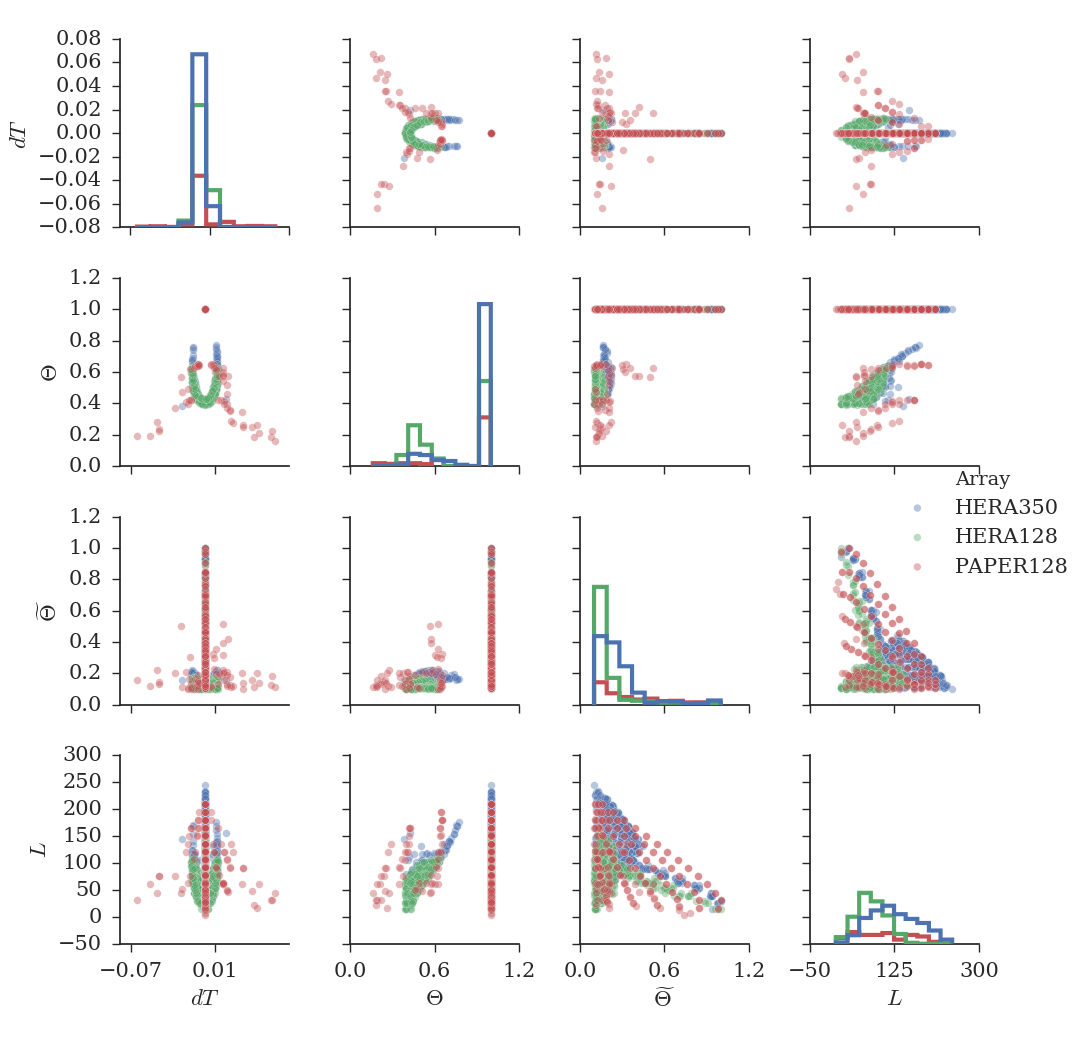
\includegraphics[width=\linewidth]{pairplot}

\caption{Pairplots of the top contributing baseline pairs in three arrays. Plotted properties are optimal time delay $dT$,  effective weight $\widetilde{\Theta}$ and baseline length $L$. Only those points with $\widetilde{\Theta}>0.01$ are shown (the weight for the top class of equivalent pair is normalized to 1). Only one baseline length is shown since all top contributing pairs have very similar lengths as expected. The scatter plots are shown with transparency so that darker regions indicate degeneracies. Scatter points of the 3 arrays overlap, in order indicated by the legend. }
\label{fig:pairplot}
\end{figure}

In Fig. \ref{fig:pairplot} we present pair-distributions of 3 different properties for baselines that contribute well to the sensitivity ($\widetilde{\Theta}>0.01$, where again the weight for the top class of equivalent pair is normalized to 1). The properties shown are effective weight $\widetilde{\Theta}$, optimal time offset $dT$, and average baseline length $L$. We only show 3 of the mentioned arrays for visual clarity. The other two results are similar barring intuitive differences. We discuss each cross-distribution plot:
\begin{itemize}

\item $dT$ vs. $\widetilde{\Theta}$:
This relation  is familiar from Fig. \ref{fig:sensplot}. The points at $dT=0$ are the equivalent baselines. Note PAPER128 has more data points with high $dT$. 

\item $dT$ vs. $L$:
PAPER128 shows the trend that longer baselines correspond to lower $dT$. HERA arrays do not exhibit this trend here because of a selection effect. Only baseline pairs with $\widetilde{\Theta}>0.01$ are shown. Shorter HERA baselines require much longer $dT$ to overlap, partly because of the hexagonal structure requires $60\degree$ of rotation to overlap baselines, partly because of the smaller primary beam. Thus most short HERA baseline pairs are not shown in this figure.


\item $\widetilde{\Theta}$ vs. $L$:
The general trend to be seen here is that longer baselines tend to have lower $\widetilde{\Theta}$. This is due to the lower multiplicity of longer baselines. The trend is particularly obvious in the linear structure for the HERA arrays, which are the equivalent baselines. Since they all have the unity $\Theta$ by definition, the linearly decreasing trend of $\widetilde{\Theta}$ is a direct measure of the baseline multiplicity structures of the HERA array configurations.

\item The top nearly equivalent pairs in HERA the same $\Theta$ (not shown) as in PAPER128, but much lower $\widetilde{\Theta}$. This is because they are longer baselines with lower multiplicity. In the end these baseline classes still lead to high contributions to total sensitivity (Fig. \ref{fig:osens}) because there are a lot more such baseline pairs for HERA.  

\end{itemize}

Having quantified the sensitivity from a given pair of baselines, we study the cumulative sensitivity of the array depending on which baseline pairs we include. Evidently we should prefer the pairs with larger $\widetilde{\Theta}$. In Fig. \ref{fig:osens} we plot $\rho$ against the minimum $\widetilde{\Theta}$. $\rho(\widetilde{\Theta}_{min})$ is the sensitivity of the array when baseline-pairs that have $\widetilde{\Theta}>\widetilde{\Theta}_{min}$ are included. The dashed lines represent the values when only the equivalent baseline-pairs are used.  We see as expected that in all cases using the nearly equivalent baselines lead to more and more significant improvements with lower $\widetilde{\Theta}_{min}$, or in other words when more baseline pairs are used. The small HERA37, with no gap (like in HERA350) or short nearly equivalent baselines (like in PAPER 128), will not benefit much from the nearly equivalent baselines. The maximum benefits for other cases are expected to be around $20\%$ to $60\%$. PAPER128 is designed with highly redundant nearly equivalent baselines, and thus  these baselines start contributing at higher $\widetilde{\Theta}_{min}$, but the gapped HERA configurations will benefit even more from nearly equivalent baselines at low $\widetilde{\Theta}_{min}$ due to the presence of more classes of such pairs. Note that here we normalized $\rho$ such that the contribution of the top equivalent baseline pair, such as are 1. This plot therefore does not compare the absolute sensitivity across the different arrays. The stepwise pattern is characteristic of a regular grid; as we step to lower $\widetilde{\Theta}$ large groups of baseline pair classes get included in ``batch''. 
%\begin{centered}
\begin{figure}[H]
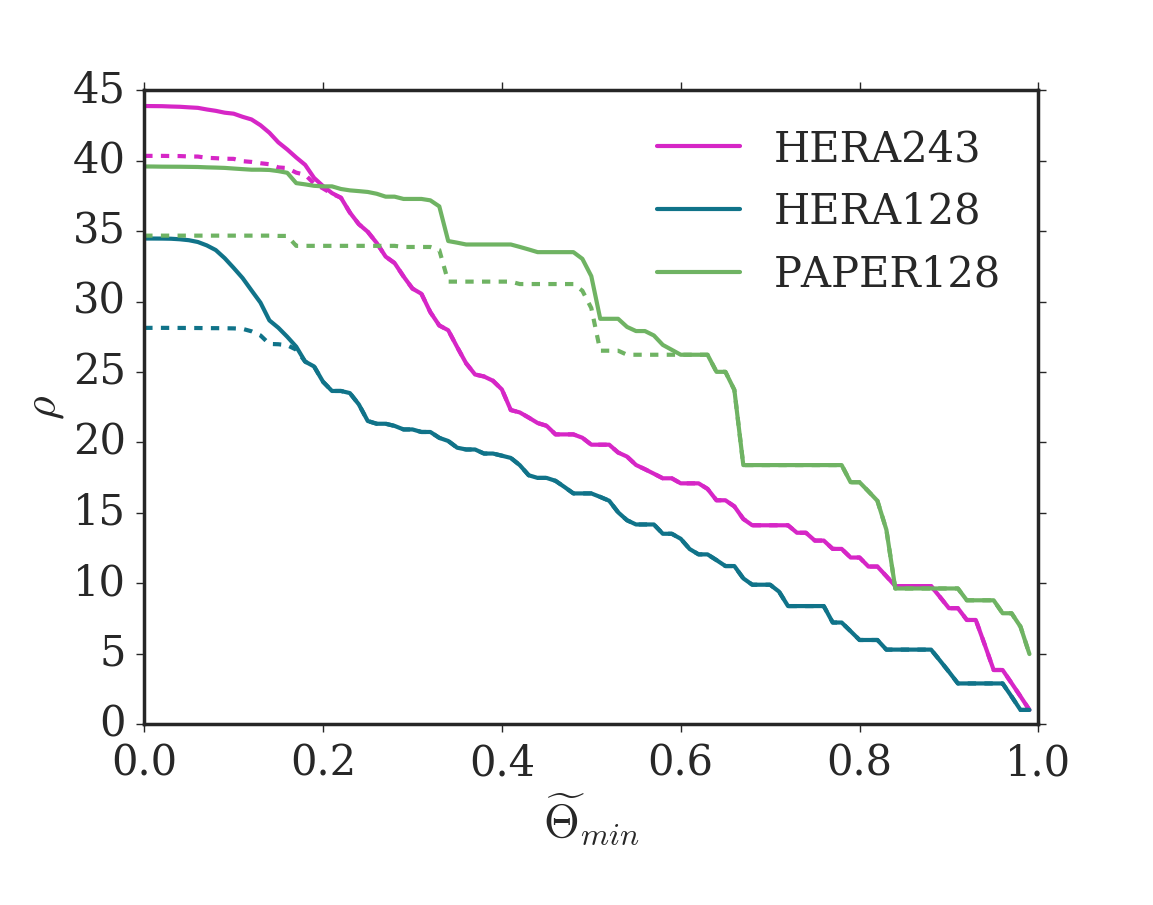
\includegraphics[width=\linewidth]{osens}
\caption{Sensitivity of redundant arrays as a function of the minimum effective weight. Dashed lines represent when only equivalent baseline pairs are used, while solid lines indicate use of both the equivalent and nearly equivalent baselines are used. The y-axis is normalized independently for each array such that the contribution of the top single equivalent pair class is unity, and thus does not indicate a comparison of absolute sensitivity across the different arrays shown.  }
\label{fig:osens}
\end{figure}
%\end{centered}











%\subsection{Notes on Data, Foreground and Noise}
%Unlike the simulated clean EOR signal, real data are dominated by foreground %and thermal noise, neither of which turns out to exhibit the correlation %pattern seen in Fig.  \ref{fig:numerics}. Foreground exhibits long-range %correlations and would lead to high responses at wide range of time-offsets. %Instrumental noise for different baselines/antenna-pairs, on the other hand, are uncorrelated and thus exhibit responses consistent with zero at all time offsets. 
%To illustrate, we use the second observing season of PAPER-128 data, taken from Jan. 21st to March 7th of 2014. To illustrate the effect of noise and foreground, we use the data before fringe-rate and delay filtering. 

\section{Conclusion}
Redundant arrays are designed to maximize sensitivity. Current generations of redundant radio arrays, such as those probing the power spectrum of the epoch of reionization could benefit from data analysis techniques that improve the sensitivity. We present a visibility and delay-transform based method of cross-multiplying baselines that are close in length and orientation to each other, thereby extracting the sensitivity contained in such partial redundancy. Our discussion focuses on drift-scan arrays but also provide the analogous expressions for tracking measurements. Our method relies on cross-multiplications of visibilities at a time-offset. For drift-scan arrays, the movement of zenith during this time-offset requires a frequency-dependent rephasing prior to delay transform. We show that such zenith-rephasing lead to manageable chromatic leakage. Given an antenna array configuration, our method identifies the best baseline pairs to cross-multiply and predict the optimal time-offset $\Delta T$, weight $\Theta$ and rephase delay $\Delta\tau$. With the predicted results one can incorporate partial redundancy into existing delay-tranform based power-spectrum pipelines through a few steps. 1). Rephase the visibilities prior to delay transforming by $\Delta\tau$. 2). Shift the visibilities in time by $\Delta T$. 3) Cross multiply the visibilities of the two baselines  to form the power spectrum. 4) combine the different baseline pairs by appropriate inverse-variance weighting that takes into account the predicted sensitivity contributions of each case. We showed that incorporation of partial redundancy accounts for $20\%$ to $60\%$ sensitivity for various configurations of PAPER and HERA. 


\pagebreak



\appendix
\section{\\Track-crossing and $w$-term \label{sec:appA}}
\label{sec:appA}
In this section we link our results from Section \ref{sec:method} to the traditional views of rotation synthesis and in particular $uv$ tracks. 
Typical convention of rotation synthesis has rotation operates on $\boldsymbol{b'}$ instead of $\hat{\boldsymbol{s}}$, in which case Eq. \eqref{eq:Theta} becomes
\begin{equation}
\Theta \equiv\int\frac{d\Omega d\nu}{X^{2}Y}|A^{*}(\hat{\boldsymbol{s}},\nu)A(\Gamma\hat{\boldsymbol{s}},\nu)||\phi(\nu)|^{2} e^{-i2\pi\frac{\nu}{c}\hat{\boldsymbol{s}}\cdot\left(\boldsymbol{b}-\widetilde{\Gamma}\boldsymbol{b'}\right)}, 
\label{eq:drift}
\end{equation}
where $\widetilde{\Gamma}$ is the inverse of $\Gamma$. 
For tracking elements, $\Gamma$ becomes a rotation around zenith:
\begin{equation}
\Theta \equiv\int\frac{d\Omega d\nu}{X^{2}Y}|A^{*}(\hat{\boldsymbol{s}},\nu)A(\hat{\boldsymbol{s}},\nu)||\phi(\nu)|^{2} e^{-i2\pi\frac{\nu}{c}\hat{\boldsymbol{s}}\cdot\left(\boldsymbol{b}-\widetilde{\Gamma}\boldsymbol{b'}\right)}, 
\label{eq:tracking}
\end{equation}

Track-crossing corresponds to vanishing of the exponent
\[
 \boldsymbol{b}-\widetilde{\Gamma}\boldsymbol{b'} = 0. \label{eq:trackcross}
 \]
If exponent vanishes, $\Theta_{\nu}$ is real, and one would not observe any non-zero phase at the peak. However, with inclusion of the $w$-term, we see that track crossings in $uv$-plane do not actually imply crossing in the $uvw$ space, therefore the exponent Eq. \eqref{eq:trackcross} does not vanish and we observe non-zero, frequency dependent peak phases even in the case of tracking arrays, as shown in Fig. \ref{fig:phi_nu}. 

Furthermore, in the case of drift-scan arrays, even a crossing in $uvw$ space does not necessarily correspond to the maximum of correlation. From Eq. \eqref{eq:drift}, we see the track-crossing condition Eq. \eqref{eq:trackcross} maximizes $\Theta$ if and only if no other term in the integral depends on $\Gamma$. We see that this is true for the tracking case (Eq. \eqref{eq:tracking}), but not the drift-scan case (Eq. \eqref{eq:drift}). Only in the special case of a tracking measurement, where the $w$-term happens to be negligible, do $uv$-track crossings correspond exactly to maxima of correlations. Incidentally, at the crossing points the exponent in Eq. \eqref{eq:trackcross} vanishes and $\psi_\nu$ is zero for all $\nu$. In general, second order effects due to the presence of $w$ is observed for the tracking measurements as in Fig. \ref{fig:phi_nu}. 


\section{\label{sec:appB}\\Derivation of Noise Covariance \label{sec:appB}}
\label{sec:appB}
In this appendix we give a brief derivation of the effective weight quoted in \ref{sec:sensitivity}. We combine the power spectrum measurements from distinct baseline classese by inverse variance weighting. We separate the visibility and power spectrum into signal and noise contributions:
\begin{equation}
\begin{aligned}
V &= V_S+V_N,\\
P &= P_S+P_N.
\end{aligned}
\end{equation}
We write the noise variance of power spectrum and visibility as:
\begin{equation}
\begin{aligned}
\sigma_V^2 &= \langle |V_N|^2 \rangle,\\
\sigma_P^2 &= \langle P_N^2 \rangle.
\end{aligned}
\end{equation}
One may notice that we have used a single covariance for the complex visibility. It is straightforward to show that the same result holds if a separate real and imaginary components are used, as long as they are independent of each other. In fact, for simplicity and without loss of generality we shall treat the visibility as a real quantity in the rest of this derivation. 
Note that though we can assume $\langle V_N^{odd-power}\rangle=0$, the same is not true for $P_N$. 

The variance of $P$ constructed with visibilities $V_1$ and $V_2$ from two baseline classes can be estimated\footnote{We assume all noise terms to be independent for simplicity, in practice the correlation of different measurements ifrom equivalent baselines are alleviated by grouping the baselines in the class and the days of observation, as in \cite{Ali2015}}:
\begin{equation}
\begin{aligned}
\sigma_P^2 &= \langle P^2\rangle -\langle P \rangle^2,\\
&\propto \langle \frac{(V_{1S}+V_{1N})^2 (V_{2S}+V_{2N})^2}{\Theta^2} \rangle - \langle \frac{(V_{1S}+V_{1N}) (V_{2S}+V_{2N})}{\Theta} \rangle ^2,\\
&= \frac{1}{\Theta^2} \left( V_{1S}^2\sigma_{V2}^2+V_{2S}^2\sigma_{V1}^2+\langle V_{1N}^2 V_{2N}^2\rangle\right), \\
&= \frac{1}{\Theta^2} \left[ V_{S}^2(\sigma_{V2}^2+\sigma_{V1}^2) + \sigma_{V1}^2 \sigma_{V2}^2\right], 
\end{aligned}
\end{equation}
where in the second last line we have substituted in the visibility noise variance. In the final line we used Wick's theorem and the fact that the signal from the two visibilities are equal. 

Recall from the discussion on multiplicities we can write
\begin{equation}
\sigma_V^2=\frac{\sigma_0^2}{M},
\end{equation}
where $\sigma_0$ is the single-baseline noise level. Letting $\rho_0=V_S^2/\sigma_0^2$ be the signal to noise ratio for a single baseline, we can write

\begin{equation}
\begin{aligned}
\sigma_P^2 & \propto  \frac{\sigma_0^4}{\Theta^2} \left[ \rho_0 \left(\frac{1}{M_1}+\frac{1}{M_2} \right) + \frac{1}{M_1 M_2}\right], \\
&\propto \frac{1}{\widetilde{\Theta}_{12}^2}.
\end{aligned}
\end{equation}
Thus we have defined a slightly modified version of the effective weight in Eq.  \eqref{eq:tildereal}:
\begin{equation}
\widetilde{\Theta}_{12}=\frac{\Theta_{12}\sqrt{M_1M_{2}}}{\sqrt{1 + \rho_0 \left(M_1+M_{2} \right)}}.
\end{equation}







\bibliographystyle{apj}
%\nocite{*}
\bibliography{draft_working}

\end{document}